\section{M\'EMOIRE SCIENTIFIQUE}
\label{sec:memoire}

\ANRinfo{Maximum 5 pages. On donne ci-dessous des indications sur le contenu possible du mémoire. Ce mémoire peut être accompagné de rapports annexes plus détaillés.\\}

\ANRinfo{Le mémoire scientifique couvre la totalité de la durée du projet. Il doit présenter une synthèse auto-suffisante rappelant les objectifs, le travail réalisé et les résultats obtenus mis en perspective avec les attentes initiales et l’état de l’art. C’est un document d’un format semblable à celui des articles scientifiques ou des monographies. Il doit refléter le caractère collectif de l’effort fait par les partenaires au cours du projet. Le coordinateur prépare ce rapport sur la base des contributions de tous les partenaires. Une version préliminaire en est soumise à l’ANR pour la revue de fin de projet.\\} 

\ANRinfo{Un mémoire scientifique signalé comme confidentiel ne sera pas diffusé. Justifier brièvement la raison de la confidentialité demandée. Les mémoires non confidentiels seront susceptibles d’être diffusés par l’ANR, notamment via les archives ouvertes http://hal.archives-ouvertes.fr.
}

\subsection*{Mémoire scientifique confidentiel :  non}

\subsection{Résumé du mémoire}

\subsection{Enjeux et problématique, état de l’art}
\ANRinfo{Présenter les enjeux initiaux du projet, la problématique formulée par le projet, et l’état de l’art sur lequel il s’appuie. Présenter leurs éventuelles évolutions pendant la durée du projet (les apports propres au projet sont présentés en C.4).}

\subsection{Approche scientifique et technique}

\subsection{Résultats obtenus}
\ANRinfo{Positionner les résultats par rapport aux livrables du projet et aux publications, brevets etc. Revisiter l’état de l’art et les enjeux à la fin du projet.}

\jordi{Où est-ce qu’on parle de l’arrêt de la thèse de Rim ?}
\mathieu{Où est-ce qu’on l'on parle (si l'on en parle) de l'arrêt maladie d'Erwan de 4 mois}

Exemple de citation pour test biblio \citep{Luc_RS}, \citep{Luc_IGARSS22}, \citep{Luc_IGARSS21} \citep{isprs-archives-XLIII-B2-2020-703-2020} \citep{Stocker_ISPRS20} \citep{Hermann_ISPRS22} \citep{Nico_RSL} \citep{GIRYFOUQUET2021320}

\subsubsection{MMDC - Multi Modal Data Cube}
Les travaux du WP1 ont été organisés autour de 3 axes : le développement de l’architecture du modèle MMDC, la préparation de jeux de données de pré-entraînement et l’intégration du pipeline d’inférence dans la chaîne $\iota^2$.
\begin{figure}
\begin{center}
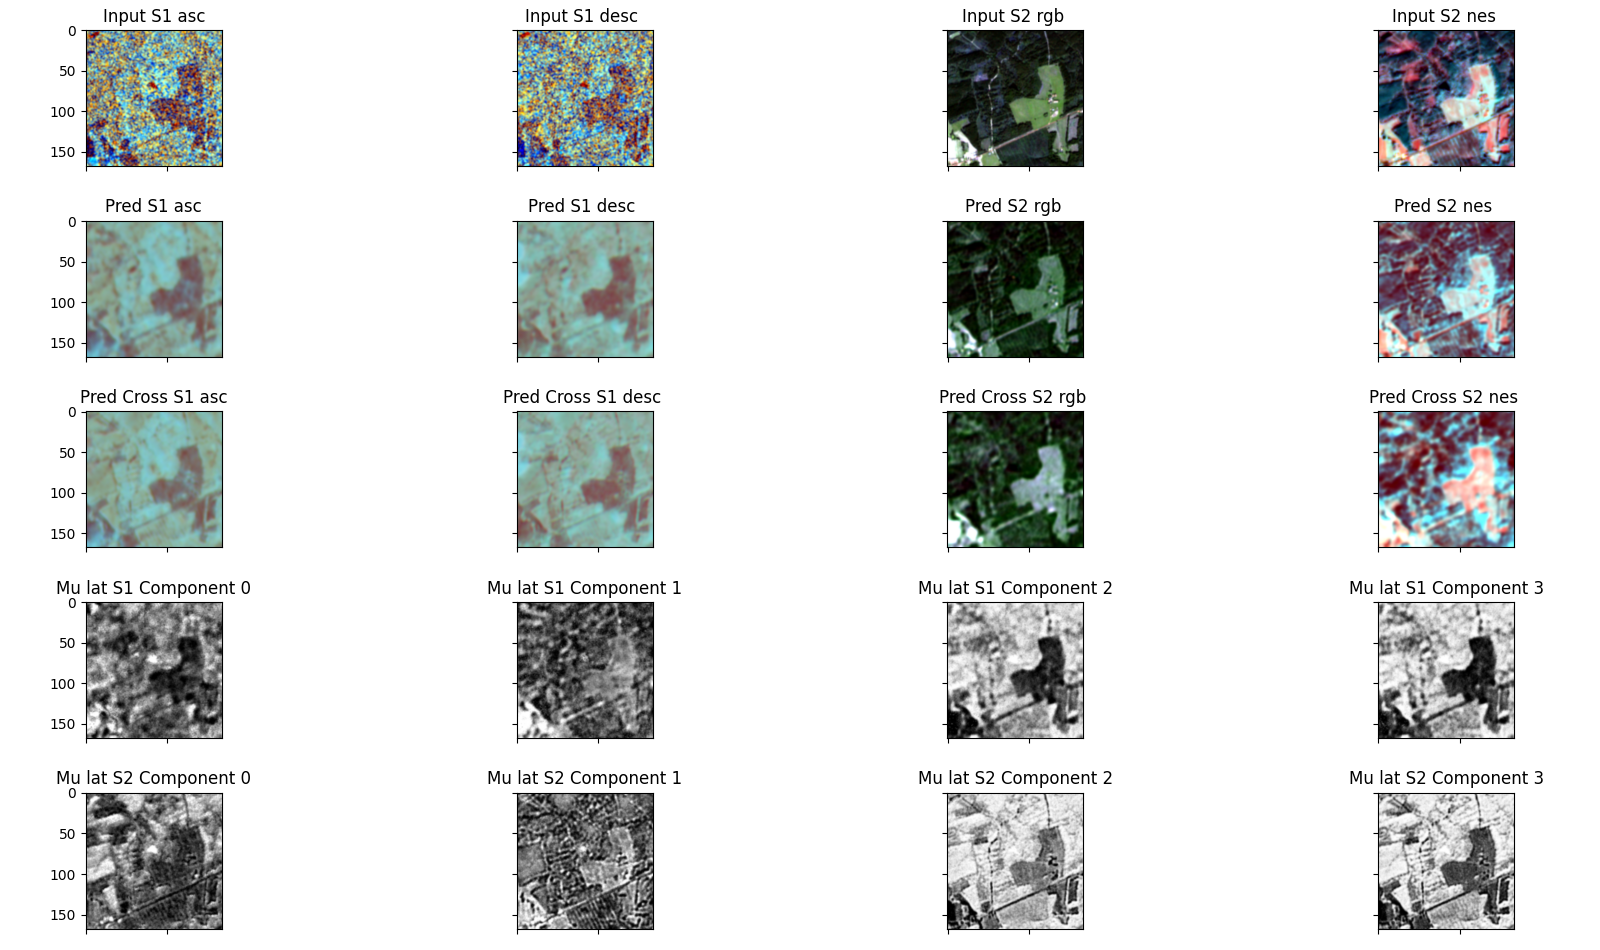
\includegraphics[width=\columnwidth]{img/wp1/mmdc5.png}
\caption{Illustration des données produites par le modèle MMDC. En colonnes, de gauche à droite, image Sentinel-1 ascendante, image Sentinel-1 descentante, image Sentinel-2 (RVB) et image Sentinel-2 (IR). En lignes, de haut en bas, données originales, réconstructions directes, reconstructions latentes, espace latent Sentinel-1 et espace latent Sentinel-2.}
\label{fig:mmdcresults}
\end{center}
\end{figure}

\paragraph{Architecture du modèle}
Le modèle MMDC retenu est un auto-encodeur variationnel multi-modal, similaire à la méthode de cross-génération de \cite{shi-2019-variat-mixtur}. Un encodeur par modalité est utilisé afin d’engendrer un espace latent gaussien. Un décodeur par modalité est aussi utilisé por réconstruire les données d’entrée. Les décodeurs peuvent être des réseaux de neurones ou des modèles physiques sans entrainement. Dans ce dernier cas, l’espace latent représente les variables d’entrée des modèles physiques. Dans le cas où les décodeurs sont des réseaux de neurones, l’espace latent n’a pas d’interprétation. Une illustration de ce dernier cas est donnée sur la figure \ref{fig:mmdcresults}.

L’entraînement du modèle se fait par optimisation d’une fonction de coût composée de 5 termes :
\begin{itemize}
\item 2 termes correspondant aux erreurs de réconstruction directes (encodage S1 suivi de décodage S1, et de même pour S2) ;
\item 2 termes correspondant aux erreurs de réconstruction croisées (encodage S1 suivi de décodage S2, et son réciproque) ;
\item 1 terme de divergence entre les espaces latents générés par les 2 encodeurs pour une paire de données S1 et S2.
\end{itemize}

Les erreurs de réconstruction sont mesurées par une log-vraisemblance gaussienne et la divergence entre les espaces latents est mesurée avec la divergence de Kullback-Leibler entre les distributions (gausiennes) inférées par les encodeurs. On se rapproche ainsi du ELBO classique dans les VAE adapté pour le cas multi-modal et où l’espace latent de chaque modalité agit en tant que prior de la modalité complémentaire.

Il est intéressant de noter la donnée S1 est composée des orbites ascendante et descendante de la même date (à 12h d’écart). Dans le cas où une seule orbite serait disponible (hors Europe, le plan d’acquisition de S1 ne garantit pas la présence des 2 images) la donnée est mise à zéro en utilisant la stratégie de modality dropout \cite{neverova-2016-moddr}.

Les données satellite sont constituées des mesures (bandes spectrales optiques et polarisations SAR), mais aussi des informations de géométrie d’acquisition (angles capteur et solaires en optique et angle d’incidence locale en SAR). Ces données sont complétées par des informations de topographie (altitude, pente et aspect issus du modèle numérique de terrain SRTM) et des variables climatiques de la base de données Worldclim 2 \cite{fick17_world}.

\paragraph{Préparartion de jeux de données multimodaux de pré-entraînement}

L’entraînement de modèles de fondation du type MMDC nécessite des gros volumes de données. Nous avons constitué un jeu de données dont le volume dépasse les 2TB. Il est composé de toutes les données disponibles sur l’année 2018 pour les capteurs Sentinel-1 et Sentinel-2 sur 50 tuiles de la grille MGRS sélectionnées de façon aléatoire sur l’ensemble des surfaces continentales de façon à couvrir des zones climatiques et des paysages différents. Elles sont illustrées sur la figure \ref{fig:mmdctiles}. Sur chacune de ces tuiles, 5 régions d’intérêt (ROI) de 1024 $\times$ 1024 pixels (à 10 m. de résolution spatiale) sont découpées de façon aléatoire. Toute la profondeur temporelle est conservée. Chaque ROI est accompagnée des 103 variables climatiques Worldclim2 et du MNT SRTM. Le code source utilisé pour la constitution du jeu de données est disponible \href{https://src.koda.cnrs.fr/mmdc/mmdc-datacollection}{en ligne}.


\begin{figure}
\begin{center}
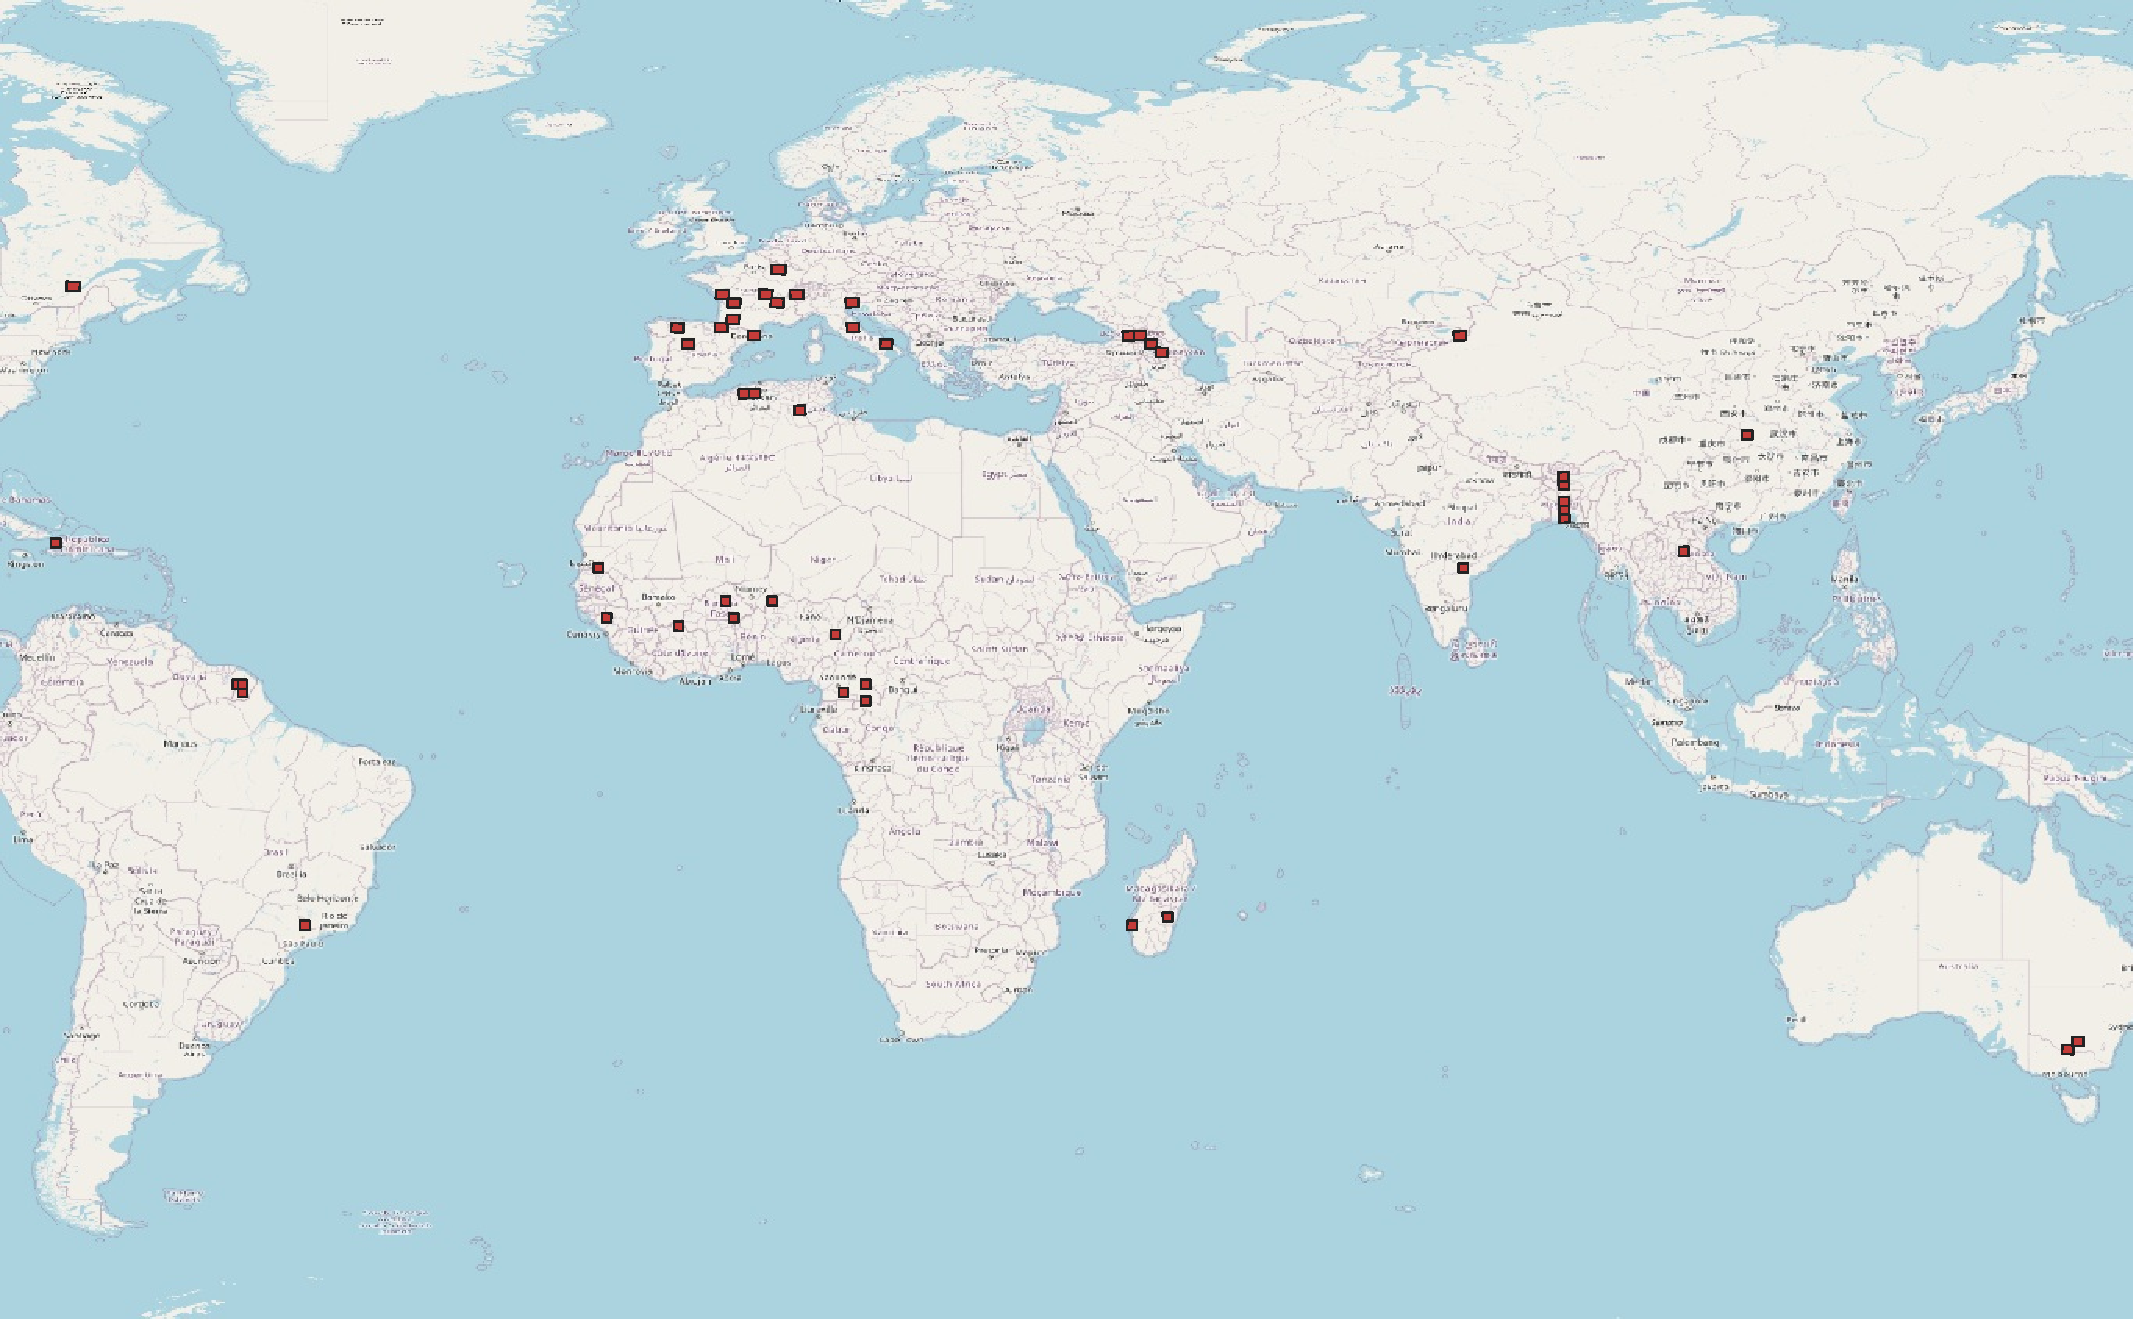
\includegraphics[width=\columnwidth]{img/wp1/tiles.pdf}
\caption{Localisation des 50 tuiles MGRS sélectionnées pour le jeu de données MMDC.}
\label{fig:mmdctiles}
\end{center}
\end{figure}

Au delà des travaux prévus dans MAESTRIA, ces données ont pu être valorisées dans \citep{dumeur-2023-self-satel}.

\paragraph{Code source}
L’ensemble du code dévelopé dans le cadre du WP1 est disponible en ligne sur \href{https://src.koda.cnrs.fr/mmdc}{Koda CNRS} . Nous avons utilisé la bibliothèque \href{https://pytorch.org/}{Pytorch} pour la mise en œuvre des modèles de réseaux de neurones, l’orchestration des apprentissages a été faite avec la bibliothèque \href{https://lightning.ai/}{Pytorch Lightning} et toutes les expériences ont été configurées et paramétrées avec la bibliothèque \href{https://hydra.cc/}{Hydra}.

Le code a été décomposé en plusieurs dépôts, dont \href{https://src.koda.cnrs.fr/mmdc/mmdc-singledate}{le principal} contient les modèles de réseaux de neurones.

Nous avons aussi réalisé le portage en Pytorch du modèle de transfert radiatif PROSAIL \cite{jacquemoud-2009-prosp-sail-model} à partir de sa version Numpy \cite{domenzain19}. Ceci a été nécessaire pour pouvoir insérer le modèle physique dans les modèles d’apprentissage profond. En effet, pour réaliser l’apprentissage de bout en bout, il est nécessaire de rétro-propager les gradients des fonctions de coût à travers toutes les opérations du modèle (encodeurs et décodeurs). Dans le cas de l’apprentissage avec priors physiques, le décodeur est remplacé par le modèle physique, qui doit être différentiable et capable de propager les gradients.

\paragraph{Intégration dans $\iota^2$}
Afin de pouvoir déployer les modèles MMDC sur de grandes étendues, MAESTRIA a proposé de faire des évolutions à la chaîne $\iota^2$ dévelopée initialement par le CESBIO. L’idée principale a était d’utiliser les encodeurs MMDC comme extracteurs de primitives qui pourraient être insérés dans le workflow $\iota^2$ (extraction de primitives, apprentissage, inférence). $\iota^2$ étant un projet existant avec des pratiques de développement ouvertes \href{https://framagit.org/iota2-project/iota2}{sur une forge publique}, les développements nécessaires à MAESTRIA ont été découpés en tickets spécifiques :
\begin{itemize}
\item création de data-loaders pour entraîner des modèles de réseaux de neurones dans $\iota^2$ (\href{https://framagit.org/iota2-project/iota2/-/issues/194}{ticket 194});
\item prise en compte de l’échantillonnage irrégulier dans les séries temporelles (\href{https://framagit.org/iota2-project/iota2/-/issues/318}{ticket 318});
\item prise en compte d’échantillons sous forme de patchs pour les CNN (\href{https://framagit.org/iota2-project/iota2/-/issues/334}{ticket 334});
\item calcul de statistiques et standardisation des données dans les data-loaders (\href{https://framagit.org/iota2-project/iota2/-/issues/418}{ticket 418});
\item profilage et opitimisation des fonctinnalités d’apprentissage profond (\href{https://framagit.org/iota2-project/iota2/-/issues/579}{ticket 579}).
  
\end{itemize}


\subsubsection{Apprentissage grande échelle}
Les travaux du WP2 concernaient le développement d'une méthode d'apprentissage adapté au contexte MAESTRIA: multi-source, grande échelle spatiale et volume de données massif. En particulier, nous avions comme objectif de gérer des données d'apprentissage bruitées (avec des labels incorrects) et de pouvoir extraire des informations statistiques des classe (e.g., multi-modalité et variabilité spatiale).

Les travaux se sont orientés vers la définition d'un algorithmes semi-supervisé permettant d'exploiter le volume important de données satellites disponibles, avec ou sans label. Comme hypothèse de départ, nous avons supposé qu'un clustering non-supervisé des données dans le domaine spectral était disponible. C'est à dire que pour chaque pixel à traiter, la probabilité d'appartenance à \(K\) clusters \(S\) était disponible. Cette hypothèse correspond à un modèle de mélange classique dans la littérature:

\[p(\mathbf{x}) = \sum_{j=1}^Kp(X=\mathbf{x}|S=j)p(S=j).\]

Un fois les clusters supposés connus, le problème d'apprentissage revient à estimer la probabilité \(r_{ij}\) qu'un cluster \(j\) appartient à la classe \(i\), avec \(i\in\{1, \ldots,k\}\). L'idée sous jacente était d'exploiter la structure par clusters des données pour limiter l'effet d'échantillons mal labélisé dans la bases de données, en réalisant une classification des densités de probabilité (les clusters) plutôt que de leur réalisation (les pixels, dont les outliers).

En utilisant le modèle \emph{robust mixture discriminant analysis} (RMDA) de~\cite{bouveyron-2009-robus-super}, il est possible d'estimer \(r_{ij}\) en minimisant la log-vraisemblance du modèle RMDA:
\begin{eqnarray}
  \label{eq:ll}
  \begin{array}{rl}
    \displaystyle{\min_{\mathbf{R}}}
   &\displaystyle{\sum_{\ell=1}^n -\ln\big(\boldsymbol{\beta}_\ell^\top\mathbf{R}\boldsymbol{\psi}_\ell\big)}\\
   \text{Constraint to} & \mathbf{R}^\top\mathbf{1}_C = \mathbf{1}_K,\\
  & \mathbf{R} \succcurlyeq 0,
  \end{array}
\end{eqnarray}
où \(\boldsymbol{\psi}_\ell\) est le vecteur d'appartenance au \(K\) clusters du pixel \(\ell\), \(\boldsymbol{\beta}_\ell\) est le vecteur \emph{one-hot-encoded} d'appartenance à la classe du pixel \(\ell\) (\(\beta_{\ell i}=1\) si \(i=c_\ell\), sinon \(\beta_{\ell i}=0\)),  \(\mathbf{R}\in\mathbb{R}^{k\times K}\) la matrice des probabilités \(r_{ij}\), \(\succcurlyeq\) dénote la contrainte de non-négativité élément par élément de \(\mathbf{R}\) et \(\mathbf{1}_k\in\mathbb{R}^k\) un vecteur contenant la valeur 1.

Nous avons montré dans un premier temps que ce problème était un problème d'optimisation convexe, en calculant la matrice hessienne de~(\ref{eq:ll}) et en observant qu'elle était définie semi-positive~\citep[Section~3.1]{GIRYFOUQUET2021320}.

A partir de là, nous avons transformer ce problème d'optimisation en un problème d'optimisation par consensus en découplant le problème en sous-problèmes plus simples à résoudre et en définissant une variable globale sur laquelle la contrainte du simplex était imposée:

\begin{eqnarray}
  \label{eq:consensus}
   \begin{array}{rl}
     \displaystyle{\min_{\mathbf{R}_\ell,\mathbf{Z}}} & \displaystyle{\sum_{\ell = 1}^{n}f_\ell(\mathbf{R}_\ell)} + g(\mathbf{Z})\\
     \text{Constraint to} & \mathbf{R}_\ell - \mathbf{Z} = \mathbf{0}\ \forall \ell\in\{1,\ldots,\ n\},
   \end{array}
\end{eqnarray}
où \(f_\ell(\mathbf{R}_\ell)  = -\ln(\boldsymbol{\beta}_\ell^\top\mathbf{R}_\ell\boldsymbol{\psi}_\ell)_{+}\) pour \(\ell\in \{1,\ldots,n\}\), \((\cdot)_{+}=\max(0, \cdot)\) et \(g(\mathbf{Z})\) est définie comme la fonction indicatrice sur le simplex \(\mathcal{S}\):
\begin{eqnarray}
  g(\mathbf{Z})  =  \left\{
                      \begin{array}{rl}
                        0 & \text{ if } \mathbf{Z}\in\mathcal{S} = \{\mathbf{Z}|\mathbf{Z}\succcurlyeq 0, \mathbf{Z}^\top\mathbf{1}_C = \mathbf{1}_{K}\} \\
                        +\infty & \text{ sinon.} 
                      \end{array}
                                  \right.                                  \label{eq:simplex}
\end{eqnarray}
Cette formulation permet d'appliquer l'algorithme ADMM~\cite[Chapter~7]{boyd-2010-distr-optim}. Dans cadre, le Lagrangien augmenté s'écrit
\begin{multline}
  \mathcal{L}_{\rho}(\mathbf{R}_1,\ldots,\mathbf{R}_n,\ \mathbf{Z},\mathbf{Y}_1,\ldots,\mathbf{Y}_n) = \\ \sum_{\ell=1}^{n} \Bigg(f_{\ell}(\mathbf{R}_\ell) + \langle\mathbf{Y}_\ell, \mathbf{R}_\ell - \mathbf{Z}\rangle_F + \frac{\rho}{2}\|\mathbf{R}_\ell - \mathbf{Z}\|^2_F\Bigg) + g(\mathbf{Z}),
  \label{eq:consensus:lagrangian}  
\end{multline}
où \(\mathbf{Y}_\ell\) sont les multiplicateurs de Lagrange, \(\langle\cdot,\cdot\rangle_F\) est le produit scalaire de Frobenius entre deux matrices réelles, \(\|\cdot\|_F\) sa norme associée et \(\rho\) un paramètre de pénalité. L'algorithme itératif résultant est le suivant:
\begin{align}
  \mathbf{R}_{\ell}^{(t+1)} = {} &  \begin{aligned}[t]
    \arg\min_{\mathbf{R}_\ell}\Bigg\{ & f_{\ell}(\mathbf{R}_\ell) + \langle\mathbf{Y}_\ell^{(t)}, \mathbf{R}_\ell - \mathbf{Z}^{(t)}\rangle_F  + \frac{\rho^{(t)}}{2}\|\mathbf{R}_\ell - \mathbf{Z}^{(t)}\|^2_F\Bigg\},
  \end{aligned}\label{eq:consensus:Rl}\\
  \mathbf{Z}^{(t+1)}  = { }&   \begin{aligned}[t]
    \arg\min_{\mathbf{Z}}\Bigg\{ & g(\mathbf{Z}) + \sum_{\ell=1}^{n} \bigg(\langle\mathbf{Y}_\ell^{(t)}, \mathbf{R}_\ell - \mathbf{Z}\rangle_F   + \frac{\rho^{(t)}}{2}\|\mathbf{R}_\ell^{(t+1)} - \mathbf{Z}\|^2_F\bigg)\Bigg\},
  \end{aligned}\label{eq:consensus:Z}\\
  \mathbf{Y}^{(t+1)}_\ell = {} &\mathbf{Y}^{(t)}_\ell + \rho^{(t)}\big(\mathbf{R}_\ell^{(t+1)}-\mathbf{Z}^{(t+1)}\big), \label{eq:consensus:Y}
\end{align}
où \((t)\) indiques l'itération courante. Cet formulation est efficiente car chaque étape de mise à jours peut se paralléliser massivement, et être obtenue analytiquement. Les étapes de mises à jours sont décrites dans~\cite{GIRYFOUQUET2021320}.

Cette algorithme a été implémenté en Python avec le compilateur JIT Numba (\mathieu{Rajouter lien vers gitlab quand réparé}). Par rapport au solveur de \cite{bouveyron-2009-robus-super}, la solution proposée est jusqu'à 400 fois plus rapide. Sur un ordinateur portable standard, un problème avec 10 classes, 100 clusters et 10 millions de pixels est résolu en 20 minutes environ.

Les résultats sur des jeux de données simulés montrent une grande robustesse vis à vis du bruit dans les labels, avec un maintient des performances jusqu'à 50\% des labels corrompus. Cependant, sur des données de télédétection réelles, la tache de clustering limite les performances globales: si les clusters sont mal définies (par exemple, plusieurs classes regroupé dans un même cluster) les performances en terms de taux de bonnes classification seront faibles.

Pour pallier à cette faiblesse, nous avons avons utilisé la dérivabilité de log-vraisemblance pour inclure cette formulation dans un auto-encoder (AE) et définir une étape de clustering dans l'espace latent. Le problème d'apprentissage consiste alors à optimiser une partie du modèle avec une fonction de coût classique des AE (reconstruction) et une fonction de coût de clustering, puis d'optimiser la log-vraisemble du modèle robuste avec la formulation discuté plus haut. Nous avons obtenue une amélioration des résultats de classification, mais cependant, pas assez pour arriver à l'état de l'art.

\subsection{Exploitation des résultats}


\subsection{Discussion} 
\ANRinfo{Discussion sur le degré de réalisation des objectifs initiaux, les verrous restant à franchir, les ruptures, les élargissements possibles, les perspectives ouvertes par le projet, l’impact scientifique, industriel ou sociétal des résultats. }


\subsection{Conclusions}


